%% jan. 4, 2011  items to fix:
%% notation for math and reference to images.
%% how include eps figures.
%% make all the little figures (search for eps) in a common, nice matlab way for the
%% example filtering operations.

\chapter{Image Sampling and Aliasing}
\label{chapter:sampling}

%Sampling: going from continuous to discrete

%Upsampling and downsampling: going from a discrete signal to another discrete signal with a different sampling rate.

\section{Introduction}

In nature, most of the signals we measure (sound, light, etc.) are defined over continuous domains (time, space, etc.). In order to process them with computers we need to transform the continuous domain into a discrete one. Sampling is the process of transforming a continuous signal into a discrete one.

We need to study the following questions: What are the possible sampling patterns to sample a signal? How can we characterize the loss of information? And how do we reduce artifacts?

Understanding how information is transformed when we convert a continuous signal into a discrete signal is important because we often have to optimize two competing factors:
\begin{itemize}
    \item Maximize the amount of available information. This requires as many samples as possible.
    \item Minimize the computational cost and memory requirements. This implies that we want to minimize the number of samples we collect.
\end{itemize}

Let's consider a one-dimensional (1D) continuous time signal $\img (t)$ and its sampled version $\img \left[n \right] = \img(n T_s)$, where $T_s$ is the {\bf sampling period}. Intuitively, it is clear that in this sampling process some information will get lost. If no information was lost, then we should be able to recover the continuous signal $\img (t)$ from its sampled version $\img \left[n \right]$ by doing some kind of interpolation.  One way of ensuring that information is not lost is to decrease $T_s$, which will result in a more accurate approximation of the continuous signal $\img (t)$ at the expense of the amount of memory needed to store $\img  \left[n \right]$.  Decreasing $T_s$ will also result in an increase of the computational cost of processing the signal $\img \left[n \right]$. Therefore, it is important to choose the appropriate $T_s$. Understanding the sampling process and how to reconstruct the continuous signal is necessary as it will allow us to find the optimal sampling parameters.

\marginnote{In this chapter we will be dealing with continuous and discrete signals and their corresponding Fourier transforms.}


\section{Aliasing}


%\begin{figure}
%\[
%\begin{array}{c}
%\text{a)}
%\begin{tikzpicture}
%\begin{axis} [width=360pt,height=90pt,
%	axis x line=middle, 
%	axis y line=middle, 
%	tick align=center,
%	every axis x label/.style={at={(current axis.right of origin)},anchor=west},
%	every axis y label/.style={at={(current axis.above origin)}, anchor=north east,above=0mm},
%	xmin=0, xmax=1.05,
%	xtick={0,0.5,1},
%	xlabel=$t$,
%	ymin=-1.5, ymax=1.5,
%	ytick={-1, 0,1},
%	ylabel={$f(t)$},
%	color=black]
% \addplot+[ycomb,domain=0:1,samples=12,samples y=0] 
% ({x}, {cos(deg(2*pi*x*9/1))}); 
% \addplot[domain=0:1,samples=201,samples y=0] 
% ({x}, {cos(deg(2*pi*x*9/1))}); 
%\end{axis}
%\end{tikzpicture}
%\\
%\text{b)}
%\begin{tikzpicture}
%\begin{axis} [width=360pt,height=90pt,
%	axis x line=middle, 
%	axis y line=middle, 
%	tick align=center,
%	every axis x label/.style={at={(current axis.right of origin)},anchor=west},
%	every axis y label/.style={at={(current axis.above origin)}, anchor=north east,above=0mm},
%	xmin=0, xmax=11.5,
%	xtick={0,1,5,11,12},
%	xlabel=$n$,
%	ymin=-1.5, ymax=1.5,
%	ytick={-1, 0,1},
%	ylabel={$f \left[n\right]$}]
%\addplot+[ycomb,domain=0:11,samples=12,samples y=0] 
% ({x}, {cos(deg(2*pi*x*12/11*9/12))}); 
%\addplot[domain=0:11,samples=201,samples y=0] 
% ({x}, {cos(deg(2*pi*x*2/11))}); 
%\end{axis}
%\end{tikzpicture}
%\\
%\text{c)}
%\begin{tikzpicture}
%\begin{axis} [width=360pt,height=90pt,
%	axis x line=middle, 
%	axis y line=middle, 
%	tick align=center,
%	every axis x label/.style={at={(current axis.right of origin)},anchor=west},
%	every axis y label/.style={at={(current axis.above origin)}, anchor=north east,above=0mm},
%	xmin=0, xmax=1.05,
%	xtick={0,0.5,1},
%	xlabel=$t$,
%	ymin=-1.5, ymax=1.5,
%	ytick={-1, 0,1},
%	ylabel={$$},
%	color=black]
% \addplot+[ycomb,domain=0:1,samples=12,samples y=0] 
% ({x}, {cos(deg(2*pi*x*9/1))}); 
% \addplot[domain=0:1,samples=201,samples y=0] 
% ({x}, {cos(deg(2*pi*x*9/1))}); 
%  \addplot[domain=0:1,samples=201,samples y=0, red] 
% ({x}, {cos(deg(2*pi*x*2/1))}); 
%\end{axis}
%\end{tikzpicture}
%\end{array}
%\]
%\caption{a) Continuous signal and its samples. b) Discrete signal and the reconstructed continuous signal by interpolation. c) Superposition of continuous signal (a) and its reconstructed approximation from the discrete samples from (b).}
%\label{fig:samplingissues}
%\end{figure}


Let's first look at one example to get a sense of the type of issues that might arise when discretizing a signal. Consider the continuous signal with the form $\img (t)=\cos (wt)$ with $w=18\pi$, shown in \fig{\ref{fig:cosine_wave_before_sampling}}. The period of this signal is $T=2 \pi / w = 1/9$ (there are nine periods in the interval $t \in \left[0, 1 \right]$).


\begin{figure}
    \centerline{
        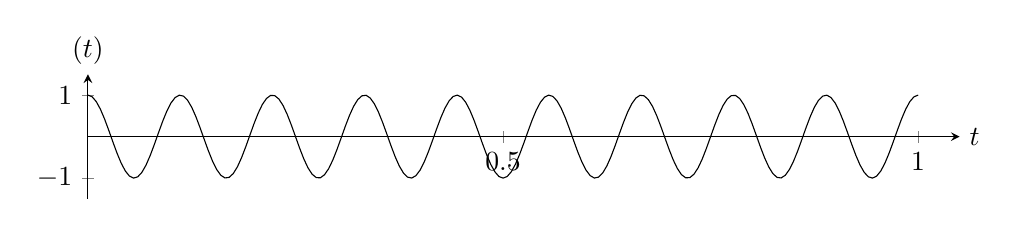
\begin{tikzpicture}
            \begin{axis} [width=360pt,height=90pt,
                    axis x line=middle,
                    axis y line=middle,
                    tick align=center,
                    every axis x label/.style={at={(current axis.right of origin)},anchor=west},
                    every axis y label/.style={at={(current axis.above origin)}, anchor=north east,above=0mm},
                    xmin=0, xmax=1.05,
                    xtick={0,0.5,1},
                    xlabel=$t$,
                    ymin=-1.5, ymax=1.5,
                    ytick={-1, 0,1},
                    ylabel={$\img(t)$},
                    color=black]
                \addplot[domain=0:1,samples=201,samples y=0]
                ({x}, {cos(deg(2*pi*x*9/1))});
            \end{axis}
        \end{tikzpicture}
    }
    \caption{Continuous cosine wave, $\img (t)=\cos (wt)$, with frequency $w=18\pi$.}
    \label{fig:cosine_wave_before_sampling}
\end{figure}



We now build a discrete signal by sampling with a period of $T_s=1/11$, which results in the discrete signal $\img  \left[n \right] = \img(n T_s)$  (there are 11 samples in the same interval $t \in \left[0, 1 \right]$). This could seem enough because there are more samples than periods. However, the samples of discrete signal, $\img  \left[n \right]$ are shown here (\fig{\ref{fig:cosine_wave_after_sampling}}):

\begin{figure}[h]
    \centerline{
        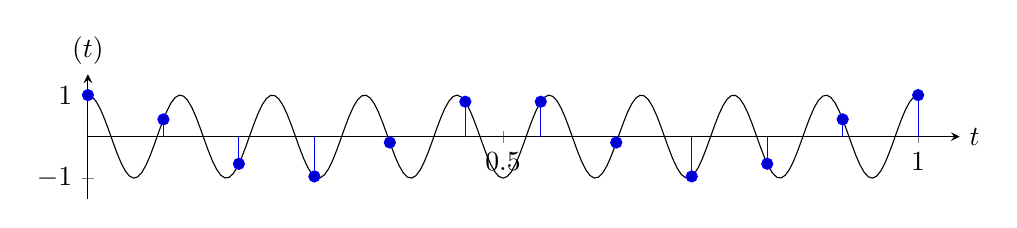
\begin{tikzpicture}
            \begin{axis} [width=360pt,height=90pt,
                    axis x line=middle,
                    axis y line=middle,
                    tick align=center,
                    every axis x label/.style={at={(current axis.right of origin)},anchor=west},
                    every axis y label/.style={at={(current axis.above origin)}, anchor=north east,above=0mm},
                    xmin=0, xmax=1.05,
                    xtick={0,0.5,1},
                    xlabel=$t$,
                    ymin=-1.5, ymax=1.5,
                    ytick={-1, 0,1},
                    ylabel={$\img (t)$},
                    color=black]
                \addplot+[ycomb,domain=0:1,samples=12,samples y=0]
                ({x}, {cos(deg(2*pi*x*9/1))});
                \addplot[domain=0:1,samples=201,samples y=0]
                ({x}, {cos(deg(2*pi*x*9/1))});
            \end{axis}
        \end{tikzpicture}
    }
    \caption{Sampling the cosine wave with a sampling period of $T_s=1/11$.}
    \label{fig:cosine_wave_after_sampling}
\end{figure}

%Figure~\ref{fig:samplingissues}.b shows $f  \left[n \right]$. 


If we now want to reconstruct the original continuous signal from its samples $\img  \left[n \right]$ there are many possibilities because the samples do not constrain what happens between samples. Therefore we will need to make some assumptions about the continuous signal. In the absence of any other prior information, we will assume that the most likely signal is the slowest and smoothest signal (we will make this assumption more precise later). Therefore, our preferred interpolation will be the one shown in red in the following plot:
\index{Slow and smooth assumption}

\begin{figure}
    \centerline{
        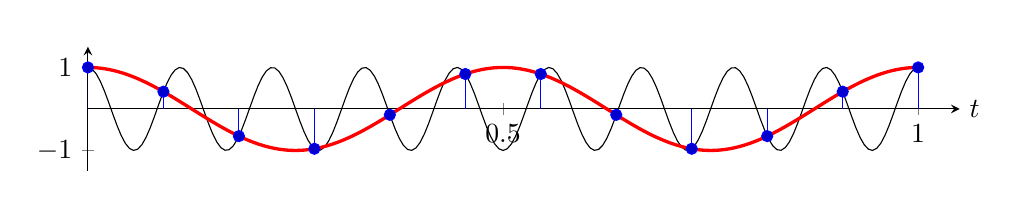
\begin{tikzpicture}
            \begin{axis} [width=360pt,height=90pt,
                    axis x line=middle,
                    axis y line=middle,
                    tick align=center,
                    every axis x label/.style={at={(current axis.right of origin)},anchor=west},
                    every axis y label/.style={at={(current axis.above origin)}, anchor=north east,above=0mm},
                    xmin=0, xmax=1.05,
                    xtick={0,0.5,1},
                    xlabel=$t$,
                    ymin=-1.5, ymax=1.5,
                    ytick={-1, 0,1},
                    ylabel={$ $},
                    color=black]
                \addplot+[ycomb,domain=0:1,samples=12,samples y=0]
                ({x}, {cos(deg(2*pi*x*9/1))});
                \addplot[domain=0:1,samples=201,samples y=0]
                ({x}, {cos(deg(2*pi*x*9/1))});
                \addplot[domain=0:1,samples=201,samples y=0, red, style=very thick]
                ({x}, {cos(deg(2*pi*x*2/1))});
            \end{axis}
        \end{tikzpicture}
    }
    \caption{There are infinite waves (only two shown) that perfectly pass by all the samples.}
\end{figure}

The plot above shows the superposition of the original signal before sampling and the reconstructed one after sampling (in red). Both signals perfectly pass through the same samples. Under the slow and smooth prior, the samples seem to correspond to a cosine function with a lower frequency (in this example $T=1/2$) than the input (which had $T=1/9$).


It is important to mention that there is nothing special about how the parameters have been chosen for this example. Many different parameter choices would have yielded the same qualitative behavior. This confusion of frequencies is called {\bf aliasing}.
\index{Aliasing}

Let's now look at an example in two dimensions (2D). As a concrete example, let's consider the 2D signal shown in \fig{\ref{fig:aliasing}}{a}. This 2D signal is a continuous function in the spatial domain defined as $\img (x,y) = \cos (w (x+2y))$ and with a frequency, $w$, which also varies with location following $w = x+2y$. That is $\img (x,y) = \cos \left( (x+2y)^2 \right)$. The image shows a set of diagonal waves with a changing frequency starting slow at the bottom left and becoming faster and faster as we approach the top-right corner.


In order to store this continuous image on a computer, we need to sample it and convert it into a discrete image, $\img \left[ n,m \right]$. \Fig{\ref{fig:aliasing}}{b} shows the resulting sampled image when the sampling rate is chosen so that it results in an image size $52 \times 52$ pixels. The first thing to note is that the resulting image keeps very little similarity to the original signal. Only the bottom-left corner of the image looks anything like the continuous signal. As we move toward the right, the image changes the dominant orientation and the frequency becomes slow again.


\begin{figure}[t]
    \centerline{
        (a)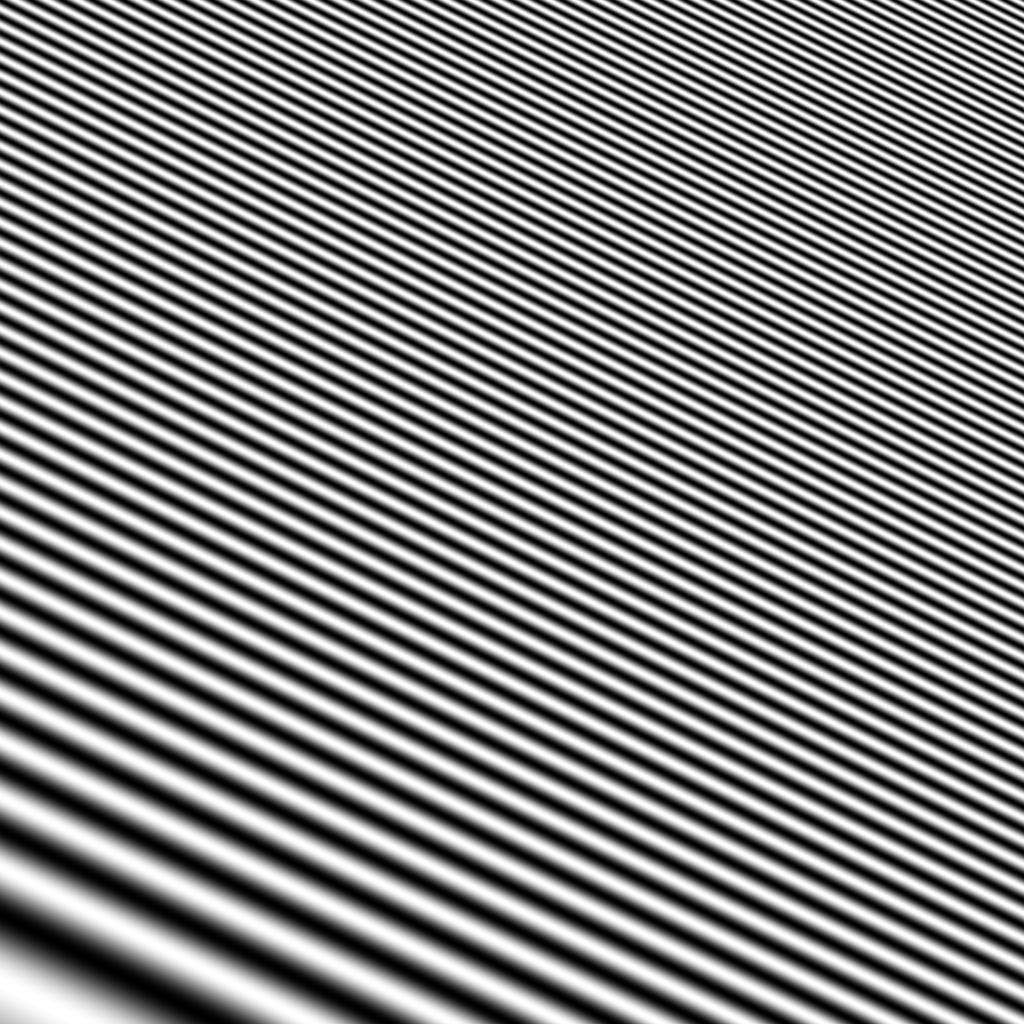
\includegraphics[width=0.45\linewidth]{figures/Image_processing_sampling/aliasing_1.jpg}
        ~
        (b)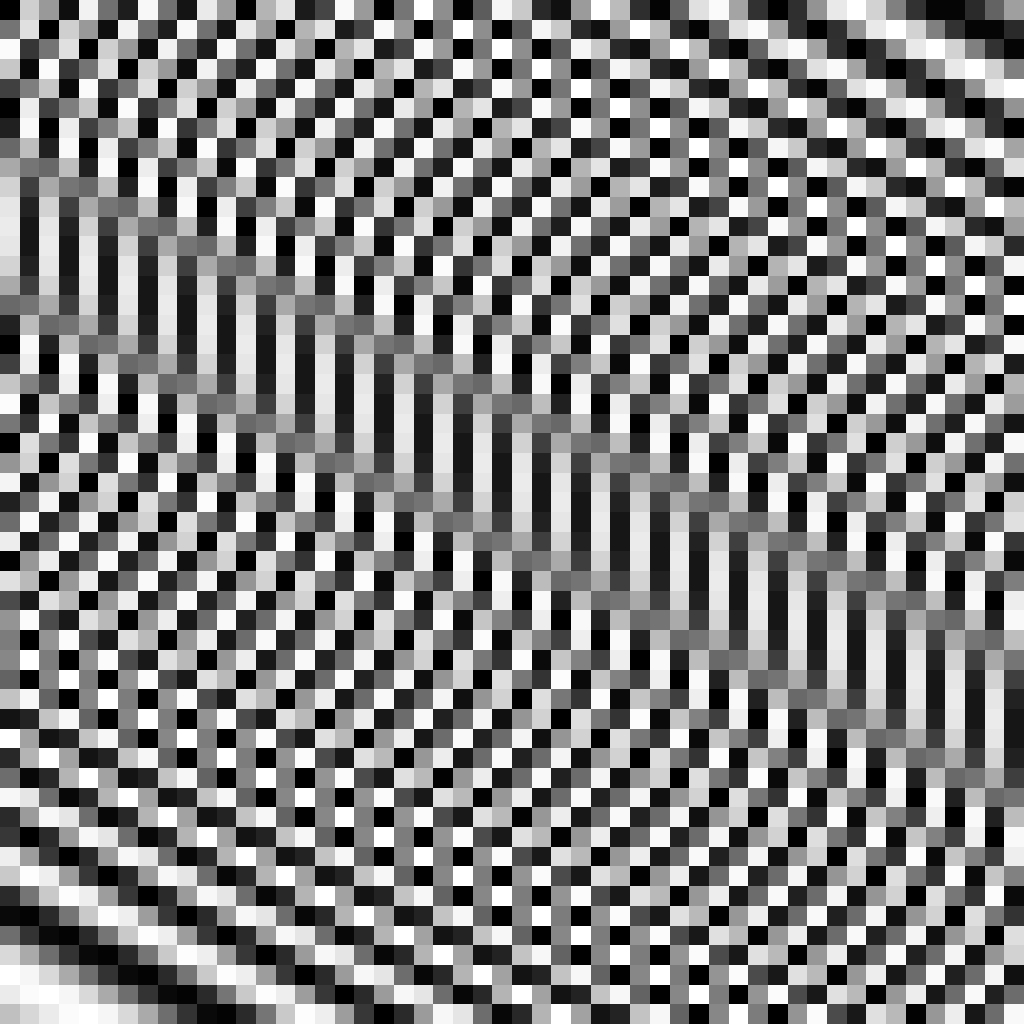
\includegraphics[width=0.45\linewidth]{figures/Image_processing_sampling/aliasing_2.jpg}
    }
    \caption{(a) A continuous image (here shown by sampling very finely). (b) Its heavily sampled version resulting in an image with size $52 \times 52$.}
    \label{fig:aliasing}
\end{figure}

\marginnote{Our perception seems to follow the slow and smooth assumption \cite{yair98}. We have prior towards smooth and slow trajectories and textures. In the presence of noise, or missing information, our visual system will tend to follow the prior.}

\section{Sampling Theorem}

Let's start by considering a band-limited signal $\img(t)$.
\index{Signals!Band-limited}
A band limited signal is a signal with no spectral content above a frequency $w_{max}$. An example of band-limited signal is a signal with the following Fourier transform:
\begin{figure}
    \centerline{
        \includegraphics[width=0.3\linewidth]{figures/Image_processing_sampling/band_limited_signal.eps}
    }
    \caption{A band-limited signal with maximum frequency $w_{max}$.}
    \label{fig:band_limited_signal}
\end{figure}

The {\bf sampling theorem} (also known as Nyquist theorem)
\index{Nyquist theorem}
states that for a signal to be perfectly reconstructed from a set of samples (under the slow and smooth prior), the sampling frequency $w_s = 2 \pi /T_s$ has to be $w_s > 2w_{max}$ when $w_{max}$ is the maximum frequency present in the input signal \cite{Shannon1948}.


The same theorem can be stated in terms of periods: the sampling period, $T_s$, has to be $T_s < T_{min} / 2$, i.e, smaller than half of period of the highest frequency component, $T_{min} = 2 \pi /w_{max}$. Note that our previous example did not satisfy the {\bf Nyquist condition}.

\marginnote{In this book we use the {\bf radian frequency} for continuous signals, $w = 2 \pi f$, where $f$ is the {\bf hertz frequency}. For a sinusoidal wave of period $T$ seconds, its frequency is $w=2\pi / T$.}[-1.1in]

One way of characterizing the sampling process is achieved by analyzing the relationship between the Fourier transform of the continuous and discrete signals.
There are many ways of finding the relationship between the two Fourier transforms. Here we will describe the most common one.

\subsection{Modeling the Sampling Process}

First, let's use the following notation. Let's denote as $\img(t)$ the continuous signal and $\img_s \left[ n \right] = f(nT_s)$ the discrete signal obtained by sampling the continuous signal. We are interested in knowing how the Fourier transform of $\img_s \left[ n \right]$ is related to the Fourier transform of $\img(t)$.

Let's start writing a model of the sampling process by defining a very special signal: the {\bf delta train} distribution (also known as the {\bf impulse train}, or {\bf Dirac comb}).
\index{Impulse train}\index{Delta train}
The delta train, $\delta_{T_s}(t)$, is a periodic signal, with period $T_s$, composed of delta impulses centered at times $nT_s$. It is defined as:
\begin{equation}
    \delta_{T_s}(t) = \sum_{n=-\infty}^{\infty} \delta(t-n T_s)
\end{equation}

When $T_s = 1$, the delta train has the following shape:

\begin{figure}
    \centerline{
        \begin{tikzpicture}
            \begin{axis} [width=360pt,height=90pt,
                    axis x line=middle,
                    axis y line=middle,
                    tick align=center,
                    every axis x label/.style={at={(current axis.right of origin)},anchor=west},
                    every axis y label/.style={at={(current axis.above origin)}, anchor=north east,above=0mm},
                    xmin=-4, xmax=7,
                    xtick={-3,...,6},
                    xlabel=$t$,
                    ymin=-0.5, ymax=1.5,
                    ytick={0,1},
                    ylabel={$\delta_{T_s}(t)$}]
                \addplot+[ycomb,mark=triangle] plot coordinates {(-3,1) (-2,1) (-1,1) (0,1) (1,1) (2,1) (3,1) (4,1) (5,1) (6,1)};
            \end{axis}
        \end{tikzpicture}
    }
    \caption{Delta train with period $T_s=1$.
        %The arrows indicate the times for which the train has an infinite value. The vertical value indicates the area of each impulse.
        The arrows show when the train's value is infinite. The height of each impulse represents its area.}
\end{figure}

The delta train can be used to model the sampling process. Remember the sampling property of the delta distribution $\img (t) \delta (t-a) = \img(a)$. If we multiply a function, $\img(t)$, by the delta train, $\delta_{T_s}(t)$, we obtain its sampled version at times $nT_s$, which we will denote as $\img_{\delta}  (t)$:

\begin{equation}
    \img_{\delta}  (t) = \img(t) \delta_{T_s}(t) = \img(t) \sum_{n=-\infty}^{\infty} \delta(t-n T_s)  =  \sum_{n=-\infty}^{\infty} \img_s \left[ n \right] \delta(t-n T_s)
\end{equation}

The two plots in \fig{\ref{fig:sampling_signal_using_train}} show a continuous function and its sampled version using the delta train.

\begin{figure}
    \centerline{
        \begin{tikzpicture}
            \begin{axis} [width=360pt,height=90pt,
                    axis x line=middle,
                    axis y line=middle,
                    tick align=center,
                    every axis x label/.style={at={(current axis.right of origin)},anchor=west},
                    every axis y label/.style={at={(current axis.above origin)}, anchor=north east,above=0mm},
                    xmin=-4, xmax=7,
                    xtick={-3,...,6},
                    xlabel=$t$,
                    ymin=-0.5, ymax=1.5,
                    ytick={0,1},
                    ylabel={$\img\left(t\right)$}]
                \addplot[smooth]
                coordinates {(-3,.2) (-2,1) (-1,.8) (0,.3) (1,.2) (2,.4) (3,.9) (4,.1) (5,.6) (6,.3)};
            \end{axis}
        \end{tikzpicture}
    }
    \centerline{
        \begin{tikzpicture}
            \begin{axis} [width=360pt,height=90pt,
                    axis x line=middle,
                    axis y line=middle,
                    tick align=center,
                    every axis x label/.style={at={(current axis.right of origin)},anchor=west},
                    every axis y label/.style={at={(current axis.above origin)}, anchor=north east,above=0mm},
                    xmin=-4, xmax=7,
                    xtick={-3,...,6},
                    xlabel=$t$,
                    ymin=-0.5, ymax=1.5,
                    ytick={0,1},
                    ylabel={$\img_{\delta} \left(t\right)$}]
                \addplot+[ycomb,mark=triangle] plot coordinates {(-3,.2) (-2,1) (-1,.8) (0,.3) (1,.2) (2,.4) (3,.9) (4,.1) (5,.6) (6,.3)};
            \end{axis}
        \end{tikzpicture}
    }
    \caption{Sampling a signal using the delta train.}
    \label{fig:sampling_signal_using_train}
\end{figure}

The delta sampled function $\img_{\delta} (t)$ is a very special function that contains the same amount of information as the discrete signal $\img_s  \left[n \right]$ but that is defined over the continuous domain $t$. In fact, the Fourier transform of $\img_{\delta} (t)$ and $\img_s  \left[n \right]$ are closely related as we will show next.

As $\img_s  \left[n \right]$ is a infinite length discrete signal, its discrete Fourier transform (DFT) is:
\begin{equation}
    \capitalimg_s(w) = \sum_{n=-\infty}^{\infty} \img_s  \left[n \right] \exp{(-jwn)}
    \label{eq:FTsampledfunction}
\end{equation}
and the continuous Fourier transform of $\img_{\delta} (t)$, an infinite length continuous signal, is:
\begin{eqnarray}
    \capitalimg_{\delta} (w) &=& \int_{n=-\infty}^{\infty} \img_{\delta} (t) \exp{(-jwt)} dt \\
    & = & \int_{n=-\infty}^{\infty} \img(t) \sum_{n=-\infty}^{\infty} \delta(t-n T_s) \exp{(-jwt)} dt \\
    & = & \sum_{n=-\infty}^{\infty} \int_{n=-\infty}^{\infty} \img(t) \delta(t-n T_s) \exp{(-jwt)} dt \\
    & = & \sum_{n=-\infty}^{\infty} \img(n T_s) \exp{(-j w n T_s)}
    \label{eq:FTdeltasampledfunction}
\end{eqnarray}
Comparing equations \ref{eq:FTsampledfunction} and \ref{eq:FTdeltasampledfunction} we see that both Fourier transforms are identical up to a scaling factor:
\begin{equation}
    \capitalimg_s(w) = \capitalimg_{\delta} \left( \frac{w}{T_s} \right).
\end{equation}

In practice, we will never directly work with the signal $\img_{\delta} (t)$, but it is a convenient construction to understand how information is transformed during the sampling process. Understanding how the sampling rate $T_s$ affects $\img_{\delta} (t)$ is equivalent to  understanding the effect that the sampling rate has in $\img_s  \left[n \right]$.

%Note that $\hat{f}  (t)$ is the product of two continuous signals. The first term is the continuous signal $f(t)$, the second term is a function composed of impulses placed at regular time instants $\delta(t-n T_s)$. The use of impulses is interesting because they are infinitely narrow in time, so the product of an impulse with a function is equivalent to taking just one sample of that function. Remember from the definition of $\delta(t)$ that $f(t) \delta(t-n T_s) = f(n T_s) \delta(t-n T_s)$. 

%$\hat{f}  (t) = f(t) \delta_{T_s}(t)$


%To see the interest of this construction, let's compute its Fourier transform. The continuous Fourier transform of $\hat{f}$ can be written as the convolution of the Fourier transforms of $f(t)$ and $\delta_{T_s}(t)$.

\subsection{Sampling in the Fourier Domain}

Now that we have seen that $\img_{\delta} (t)$ and the discrete signal $\img_s  \left[n \right]$ have similar Fourier transforms, let's compute the Fourier transform of $\img_{\delta} (t)$. Note that $\img_{\delta} (t)$ is the product of two continuous signals. The first term is the continuous signal $\img(t)$, and the second term is a function composed of impulses placed at regular time instants $\delta(t-n T_s)$. We can compute the continuous Fourier transform of $\img_{\delta} (t)$ as the convolution of the Fourier transforms of $\img(t)$ and $\delta_{T_s}(t)$.



The Fourier transform of a delta comb is:


\begin{eqnarray}
    \Delta_{T_s} (w) &=& \int_{-\infty}^{\infty}  \delta_{T_s}(t) \exp \left(-jwt\right) dw \nonumber \\
    &=&\sum_{n=-\infty}^{\infty} \int_{-\infty}^{\infty}  \delta(t-n T_s) \exp \left(-jwt\right) dw \nonumber \\
    &=&\sum_{n=-\infty}^{\infty}  \exp \left(-jwnT_s\right) \nonumber \\
    &=& \frac{2\pi}{T_s} \sum_{k=-\infty}^{\infty} \delta \left(w-k \frac{2 \pi}{T_s} \right)
\end{eqnarray}
Deriving the last step is a bit involved and we invite the readers to work out the details. The result is that the Fourier transform of an impulse train is also an impulse train but with a displacement in frequency between impulses that grows when the spacing in time decreases:

\begin{equation}
    \delta_{T_s}(t)
    \xrightarrow{\mathscr{F}}
    \delta_{\frac{2 \pi}{T_s}}(w)
\end{equation}



\marginnote{
    The delta train with period $T_s$ is: \\[6pt]
    \centerline{
        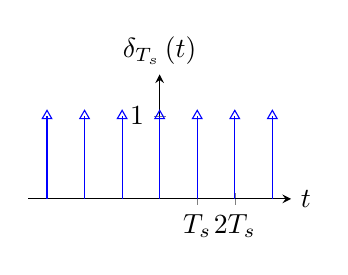
\begin{tikzpicture}
            \begin{axis} [width=140pt,height=90pt,
                    axis x line=middle,
                    axis y line=middle,
                    tick align=center,
                    every axis x label/.style={at={(current axis.right of origin)},anchor=west},
                    every axis y label/.style={at={(current axis.above origin)}, anchor=north east,above=0mm},
                    xmin=-3.5, xmax=3.5,
                    xtick={$T_s$},
                    xtick = {0, 1, 2},
                    xticklabels = {$0$,$T_s$,$2T_s$},
                    xlabel=$t$,
                    ymin=0, ymax=1.5,
                    ytick={0,1},
                    ylabel={$\delta_{T_s} \left(t \right)$}]
                \addplot+[ycomb,mark=triangle] plot coordinates {(-3,1) (-2,1) (-1,1) (0,1) (1,1) (2,1) (3,1)};
            \end{axis}
        \end{tikzpicture}
    }
    and its Fourier transform is:\\[6pt]
    \centerline{
        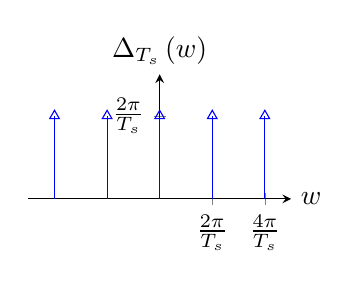
\begin{tikzpicture}
            \begin{axis} [width=140pt,height=90pt,
                    axis x line=middle,
                    axis y line=middle,
                    tick align=center,
                    every axis x label/.style={at={(current axis.right of origin)},anchor=west},
                    every axis y label/.style={at={(current axis.above origin)}, anchor=north east,above=0mm},
                    xmin=-2.5, xmax=2.5,
                    xtick={$T_s$},
                    xtick = {0, 1, 2},
                    xticklabels = {$0$,$\frac{2\pi}{T_s}$,$\frac{4\pi}{T_s}$},
                    xlabel=$w$,
                    ymin=0, ymax=1.5,
                    ytick={0,1},
                    yticklabels = {$0$,$\frac{2\pi}{T_s}$},
                    ylabel={$\Delta_{T_s} \left(w \right)$}]
                \addplot+[ycomb,mark=triangle] plot coordinates {(-2,1) (-1,1) (0,1) (1,1) (2,1)};
            \end{axis}
        \end{tikzpicture}
    }
}


Therefore, the continuous Fourier transform of $\img_{\delta} (t)$ can be written as:
\begin{equation}
    \capitalimg_{\delta} (w) = \capitalimg(w) \circ \frac{2\pi}{T_s} \sum_{k=-\infty}^{\infty} \delta \left(w-k \frac{2 \pi}{T_s} \right) = \frac{2\pi}{T_s} \sum_{k=-\infty}^{\infty} \capitalimg \left(w-k \frac{2 \pi}{T_s} \right)
\end{equation}
where $\capitalimg(w)$ is the Fourier transform of $\img(t)$. This equation shows that $\capitalimg_{\delta} (w)$ is built as an infinite sum of translated copies of $\capitalimg(w)$, as shown in \fig{\ref{fig:sketch_aliasing}}{a}. Each copy is centered on $k \frac{2 \pi}{T_s}$. If $T_s$ is small (i.e., if we sample very fast) then those copies will be far away from each other (\fig{\ref{fig:sketch_aliasing}}[a]). But if we have few samples and $T_s$ is large, those copies will get very close and will start mixing with each other (\fig{\ref{fig:sketch_aliasing}}[b]). High frequency content in $\capitalimg(w)$ will affect the low frequency content of $\capitalimg_{\delta} (w)$, and this is exactly what produces aliasing.

\begin{figure}[t]
    \centerline{
        \includegraphics[width=1\linewidth]{figures/Image_processing_sampling/sketch_aliasing.eps}
    }
    \caption{Sketch to illustrate aliasing. Example of a band-limited signal, with frequency content only inside the interval $(-w_{max}, w_{max})$. (a) Sampled with a sampling period such a that $T_s < \pi/w_{max}$. (b) Sampled with a period $T_s > \pi/w_{max}$. Aliasing is due to the overlap between the translated copies of the signal Fourier transform, $\capitalimg(w)$.}
    \label{fig:sketch_aliasing}
\end{figure}

The Nyquist limit
\index{Nyquist limit}
is reached when the maximum frequency, $w_{max}$, with spectral content in $\capitalimg (w)$ overlaps with its translated copy. This overlap occurs when the sampling period, $T_s$, is $T_s > \pi/w_{max}$. To avoid aliasing, the sampling period has to be shorter than $\pi/w_{max}$.
%$w_{max} > \pi/T_s$. 



\section{Reconstruction}

The reconstruction process consists in recovering a continuous signal from its samples by interpolation. In this section we will study what the ideal interpolation scheme is and what other practical interpolations exist.

\section{Ideal Reconstruction}
\label{sec:aliasing:ideal_reconstruction}

When the Nyquist condition is satisfied, we know that it is possible to reconstruct the original continuous signal from the samples. We just need to apply a box filter that has a constant gain for all the frequencies inside $w \in \left[-\pi / T_s, \pi / T_s \right]$, and 0 outside. The phase of the filter should be zero. That is,
\begin{equation}
    H(w) =
    \begin{cases}
        \frac{T_s}{2\pi} & \quad \text{if } w \in \left[-\pi / T_s, \pi / T_s \right] \\
        0                & \quad \text{otherwise }                                    \\
    \end{cases}
    \label{eq:boxfilterFT}
\end{equation}


%Anyway, when something is impossible, generally it is because it does not matter and it might just mean that it is not the right way of thinking about the problem. So let's not worry about it. 

The impulse response of such a filter is $h(t) = \text{sinc} (t/T_s)$ where the {\bf sinc} function is:
\begin{equation}
    \text{sinc} (t) = \frac{\sin (\pi t)}{\pi t}
\end{equation}
\index{Sinc function}

The sinc function (\fig{\ref{fig:sinc_function}}) it is an infinite length continuous signal
that has its maximum at the origin, $\text{sinc} (0)=1$, it is symmetrical, $\text{sinc} (t) = \text{sinc} (-t)$, and it is a sinusoidal wave with a period of 2 that decays in amplitude at a rate $1/t$ as shown in this plot:

\begin{figure}
    \centerline{
        \begin{tikzpicture}
            \begin{axis} [width=360pt,height=190pt,
                    axis x line=middle,
                    axis y line=middle,
                    tick align=center,
                    every axis x label/.style={at={(current axis.right of origin)},anchor=west},
                    every axis y label/.style={at={(current axis.above origin)}, anchor=north east,above=0mm},
                    xmin=-7.05, xmax=7.05,
                    xtick={-6,-5,-4,-3,-2,-1,1,2,3,4,5,6},
                    xlabel=$t$,
                    ymin=-.3, ymax=1.2,
                    ytick={-7,...,7},
                    ylabel={sinc$(t)$},
                    color=black]
                \addplot[domain=-10:10,samples=200,samples y=0]
                ({x}, {sin(deg(pi*x)) / (pi*x) });
            \end{axis}
        \end{tikzpicture}
    }
    \caption{Sinc function. This signal is a modulated sine signal with an amplitude decay of $1/t$. The frequency is normalized so that the zero crossings happen at integer values.}
    \label{fig:sinc_function}
\end{figure}

When no other prior information is available about the function $\img(t)$, and under the slow and smooth prior, this is the optimal reconstruction in terms of the L2 norm:
\begin{equation}
    \text{sinc} (t/T_s) = \argmin_{h(t)} \int \left( \img(t) - \img_{\delta} (t) \circ h(t) \right)^2 dt =
    \argmin_{h(t)} \int \left( \capitalimg(w) - \capitalimg_{\delta} (w) H(w) \right) ^2 dw
\end{equation}
Then the function, $\img_{\delta} (t)$, that best approximates the input signal from its samples is:
\begin{equation}
    \widetilde \img(t) =  \img_{\delta} (t) \circ \text{sinc} (t) = \sum_{n=-\infty}^{\infty} \img_s\left[n \right] \text{sinc} \left(\frac{t-nT_s}{T_s} \right)
\end{equation}
where $\widetilde \img(t)$ is the reconstructed signal from the samples $\img_s\left[n \right]$. The plot in \fig{\ref{fig:sampling_reconstruction2}} shows how the linear superposition of all the scaled and shifted sincs produces a smooth interpolation of the sampled function. Note how the zero crossings of each sinc coincide with the sample locations.


\begin{figure}[h]
    \centerline{
        \includegraphics[width=1\linewidth]{figures/Image_processing_sampling/sampling_reconstruction2.eps}
    }
    \caption{Smooth interpolation of the sampled function using sinc functions.}
    \label{fig:sampling_reconstruction2}
\end{figure}

% The sampling theorem is usually known as the Shannon Sampling Theorem due to Claude E. Shannon�s paper �A mathematical theory of communication� in 1948.
% The minimum required sampling rate fs (i.e. 2xB) is known as the Nyquist sampling rate or Nyquist frequency because of H. Nyquist�s work on telegraph transmission in 1924



%\begin{figure}
%\includegraphics[width=1\linewidth]{figures/Image_processing_sampling/sampling_reconstruction.eps}
%\caption{Reconstruction. a) Signal multiplied by a delta train. Each line corresponds to one impulse. The height of each impulse corresponds to the value of its integral. b) sinc function. c) magnitude of the Fourier transform of (a). d) Fourier transform of (b). The width of the box is set to cover just the central repetition of the FT shown in (c).  e) Illustration of the reconstruction process. The sinc functions are scaled and shifted on top of each sample and then summed up (only six are shown). Note how the zero crossings coincide with the sample locations. The sum of all the sinc function corresponds to the red curve.} 
%\label{fig:samplingreconstruction}
%\end{figure}


\Fig{\ref{fig:alias1d}} illustrates how the reconstruction degrades as a function of the sampling rate. In this example, there is one band-limited input signal (i.e., there is a frequency, $w_{max}$, for which the magnitude of the Fourier transform is zero for all frequencies above $w_{max}$). When we sample this signal with a sampling period of $T_s = 4$ s, in its FT we see replicates of the $\capitalimg(w)$ centered around $\pi/2$. With $T_s=8$ s, the replicates appear centered around $\pi/4$ and they start touching. Note that $T_s=8$ is slightly above the Nyquist's limit and some aliasing will exist. For $T_s=16$ aliasing is severe and information will be lost, making it impossible (without any additional prior information) to reconstruct the continuous function from its samples.



\begin{figure}
    \includegraphics[width=1\linewidth]{figures/Image_processing_sampling/sampling_FT4.eps}
    \caption{(left column)  Spatial sampling
        pattern.  (middle column)  Fourier transform of that spatial pattern,
        revealing replication locations of the Fourier
        transform spectrum of the subsampled signal.  (right column) Subsampled signal.  Zeroing out all but the central
        replication of the image spectrum yields the
        interpolated signal shown in red.
    }
    \label{fig:alias1d}
\end{figure}

\marginnote{A signal cannot be simultaneously time limited and frequency band limited. For any time limited signal (i.e., a signal that is defined inside an interval $t \in \left[a,b \right]$ and it is zero outside) the Fourier transform is not band limited.}[-1.5in]


All the derivations extend naturally to 2D because all the functions are separable along the two spatial dimensions. In two dimensions, the ideal interpolation function is:
\begin{equation}
    \text{sinc} (x,y)  = \frac{\sin (\pi x)}{\pi x} \frac{\sin (\pi y)}{\pi y}
\end{equation}

We will discuss the 2D case a bit more in detail later as sampling images opens the door to different sampling strategies beyond simply adjusting the sampling rate.

\subsection{Approximate Reconstruction with Local Kernels}

One disadvantage of the ideal reconstruction is that the $\text{sinc}$ function has infinite support which means that to interpolate each instant we need to linearly combine all the samples $\img \left[n \right]$. Sometimes it is better to have a local reconstruction that only depends on the nearby samples.

Indeed, there are other possible reconstructions that are not optimal in terms of the L2 norm, but that only require local computations.

In 1D, some of the most popular interpolation kernels are nearest interpolation, and linear. Nearest interpolation consists in assigning to each time instant the value of the nearest sample in time. Linear interpolation consist in interpolating linearly between two consecutive values.

All of them can be written as a linear convolution with a kernel $h(t)$ as shown in \fig{\ref{fig:sampling_reconstruction3}}:

\begin{figure}
    \centerline{
        \includegraphics[width=1\linewidth]{figures/Image_processing_sampling/sampling_reconstruction3.eps}
    }
    \caption{(top) Nearest interpolation. (bottom) Linear interpolation. Both interpolation methods can be modeled by a convolution with the kernel shown in the middle (a box and a triangle).}
    \label{fig:sampling_reconstruction3}
\end{figure}

The nearest neighbor interpolation is the result of the convolution of $\img_\delta (t)$ with a box of width $T_s$. The linear interpolation, the interpolation kernel $h(t)$ is a triangle of width $2T_s$.\footnote{The convolution of two box filters of width $T_s/2$ is a triangle of length $T_s$.}
Lanczos-1 interpolation
%\cite{} 
consists in using as kernel only the central lobe of the sinc function. This provides an interpolation that is smooth using only a local neighborhood. Other interpolation methods such as cubic interpolation can also be written as convolutions.
\index{Lanczos interpolation}

% Cubic interpolation:
% https://www.cs.bgu.ac.il/~dip211/wiki.files/Cubic%20Convolution%20Interpolation.pdf


\section{A Family of 2D Spatial Samplings}

Let's now analyze what happens when sampling 2D signals to form discrete images. In 2D things get more interesting. If we have a continuous image $\img (x,y)$ we can sample it using a rectangular grid as $\img_s \left[n,m \right] = \img \left(nT_x, mT_y \right)$. We can do a very similar analysis to the one we just did for the 1D case. But in 2D we can have more interesting sampling patterns. For instance, we could define the discrete image as:
\begin{equation}
    \img_s \left[n,m \right] = \img \left( an+bm, cn+dm \right)
\end{equation}
where $a,b,c,d$ are constants. For instance, if $a=T,b=0,c=0,d=T$ then we will have a regular {\bf rectangular sampling}. But we could have other patterns. For instance,  if we set $a=T_1,b=-T_2 / 2,c=0,d=T_2$ then we obtain an {\bf hexagonal sampling}. We can also place the samples at random locations ({\bf irregular sampling}). \Fig{\ref{fig:sampling_grids}} shows different sampling patterns.

\begin{figure}
    \centerline{
        \includegraphics[width=1\linewidth]{figures/Image_processing_sampling/sampling_grids.eps}
    }
    \caption{Three types of sampling: rectangular grid, hexagonal, and irregular.}
    \label{fig:sampling_grids}
\end{figure}

Now we can ask the following question: What is the optimal 2D sample arrangement given a fixed number of samples? What we want is to chose the sample arrangement that will allow the best reconstruction of the input continuous signal from a fixed number of samples. As we did with the 1D case, we can answer this question by studying the relationship between the Fourier transform of the continuous signal and the sampled one, which will reveal how aliasing happens and what sampling pattern minimizes it.

We model sampling by multiplying the continuous image by a delta train in 2D:
\begin{equation}
    \img_{\delta} (x,y) = \img \left( x,y \right) \sum_{n=-\infty}^{\infty} \sum_{m=-\infty}^{\infty} \delta \left( x- an-bm, y - cn-dm \right)
\end{equation}
%where the 2D delta train can be written as: (the impulse is separable):
%\begin{equation}
%\sum_n \sum_m \delta \left( x- an-bm, y - cn-dm \right) = \sum_n \sum_m \delta \left( x- an-bm \right) \delta \left( y - cn-dm \right)
%\end{equation}
We can simplify the notation by encoding the position as vectors, $\mathbf{x} = (x,y)^T$,  $\mathbf{n} = (n,m)^T$, and $\mathbf{A}$ is the matrix:
\begin{equation}
    \mathbf{A} = \left[
        \begin{array}{cc}
            a & b \\
            c & d
        \end{array}
        \right]
\end{equation}
where the 2D delta train can be written using vector notation for the continuous spatial coordinates:
\begin{equation}
    \delta_{\mathbf{A}}(\mathbf{x}) = \sum_{\mathbf{n} \in \mathbb{Z}^2} \delta \left( \mathbf{x} - \mathbf{A} \mathbf{n} \right)
\end{equation}



The continuous Fourier transform of this delta train can be done by applying a change in variables and then using a similar procedure as the one followed in the 1D case. The result is:
\begin{equation}
    \Delta_{A} (\mathbf{w}) = \frac{(2 \pi)^2}{|\mathbf{A}|} \sum_{\mathbf{k} \in \mathbb{Z}^2} \delta \left( \mathbf{w} - 2 \pi \mathbf{A}^{-1} \mathbf{k} \right)
\end{equation}

Therefore, the Fourier transform of the sampled signal $\img_{\delta} (x,y)$ is:
\begin{equation}
    \capitalimg_{\delta} \left( \mathbf{w} \right) =  \frac{(2 \pi)^2}{|\mathbf{A}|} \sum_{\mathbf{k} \in \mathbb{Z}^2} \capitalimg \left( \mathbf{w} - 2 \pi \mathbf{A}^{-1} \mathbf{k} \right)
    \label{eq:genericsampling}
\end{equation}
Remember that for $2\times2$ matrices the inverse is easy to write:
\begin{equation}
    \mathbf{A}^{-1} = \frac{1}{|\mathbf{A}|} \left[
        \begin{array}{cc}
            d  & -b \\
            -c & a
        \end{array}
        \right]
\end{equation}
We can now check what happens with different sampling strategies. For instance, the 2D rectangular sampling, \eqn{\ref{eq:genericsampling}}, simplifies to:
\begin{equation}
    \capitalimg_{\delta} \left(w_x, w_y \right) =  \frac{(2 \pi)^2}{T^2} \sum_{k_1=-\infty}^{\infty} \sum_{k_2=-\infty}^{\infty} \capitalimg \left( w_x - \frac{2\pi}{T}k_1, w_y - \frac{2\pi}{T}k_2 \right)
\end{equation}
This is similar to the 1D case. We leave to the reader to write down the form of the hexagonal sampling.
\index{Hexagonal sampling}



\Fig{\ref{fig:sampling_grids_FT}} shows a sketch of the Fourier transforms of the rectangular and hexagonal samplings. The region delimited by the red polygon shows the region of valid frequencies. If the input signal only has spectral content within that region, then there will be no aliasing. The optimal sampling will be the one that makes that region as large as possible for a fixed number of samples.



\begin{figure}[t]
    \centerline{
        \includegraphics[width=1\linewidth]{figures/Image_processing_sampling/sampling_grids_FT.eps}
    }
    \caption{Sketch of the Fourier transforms of the rectangular and hexagonal samplings. The red boundary denotes the spectral content that gets periodically repeated.}
    \label{fig:sampling_grids_FT}
\end{figure}

The optimal sampling strategy is the regular hexagonal sampling. This is not the sampling used in computer vision as all images are always represented on a rectangular grid, but an hexagonal sampling achieves an increase of around $10$ percent in resolution for the same amount of samples. In fact, the distribution of photoreceptors at the center of the retina \cite{Curcio87,Curcio1990} are distributed closely resembling an hexagonal array over small patches as shown in \fig{\ref{fig:samplingfovea}}.
% [Curcio,1987] C. A. Curcio, K. R. Sloan, Jr., O. Packer et al., Distribution of cones in human and monkey retina: individual variability and radial asymmetry, Science 236, 579-582 (1987).
Working with convolutional filters defined over an hexagonal grid is more efficient and it can achieve better radial symmetry \cite{Mersereau79,Simoncelli90subbandimage}.

% http://sepwww.stanford.edu/data/media/public/oldreports/sep38/38_18.pdf

%\begin{figure}
%\includegraphics[width=1\linewidth]{figures/intro_signals/sampling_rec.eps}
%\includegraphics[width=1\linewidth]{figures/Image_processing_sampling/sampling_FT3.eps}
%\caption{Sampling patterns.} 
%\label{fig:samplingpatterns}
%\end{figure}


\begin{figure}[t]
    \centerline{
        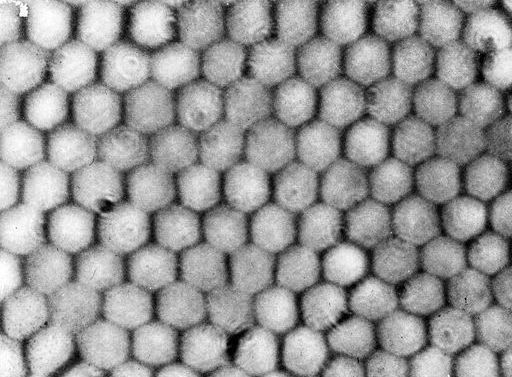
\includegraphics[width=.6\linewidth]{figures/Image_processing_sampling/sampling_fovea.jpg}}
    \caption{Distributions of cones in the fovea of a Monkey  \cite{Curcio1990}. The image shows a cross-section of the retina at the level of the photoreceptors. {\em Source:} \cite{Curcio1990}.}
    \label{fig:samplingfovea}
\end{figure}

%With all the examples and derivations in this book, we will always be working with a regular rectangular grid. 
The analysis we have presented in this chapter assumes signals of infinite length. However, images will have a finite size. The same results can be applied by extending the image to infinity with zero padding.

\section{Anti-Aliasing Filter}
\index{Filter!Anti-aliasing}

Sampling with the wrong frequency has interesting effects in 2D. \Fig{\ref{fig:aliasingFTzebra}}{a} shows an example of a picture downsampled at different resolutions (412$\times$512, 103$\times$128, 52$\times$64, and 26$\times$32) and then reconstructed to the original resolution (412$\times$512 pixels). For the figures, as we do not have access to the continuous image, we always work with sampled versions. But the original image is very high resolution and we can think of it as being the continuous image.


The images in \fig{\ref{fig:aliasingFTzebra}}{a} show the effects of aliasing. The stripes in the zebra's body change orientation as we downsample them. And for the lowest resolution image, it is even hard to recognize the animal as being a zebra. \Fig{\ref{fig:aliasingFTzebra}}{b} shows what happens with the image Fourier transform when we multiply the image with the delta train, with a one every four samples along each dimension (second column of \fig{\ref{fig:aliasingFTzebra}}[b]). \Fig{\ref{fig:aliasingFTzebra}}{c} shows the magnitude of the DFT of the sampled image (it corresponds to the region inside the green square in \fig{\ref{fig:aliasingFTzebra}}{b}. The DFT changes substantially, due to aliasing, from one resolution to the next one.


%\begin{figure}
%\includegraphics[width=1\linewidth]{figures/intro_signals/aliasing_zebra2.eps}
%\caption{Aliasing and antialiasing filter. The zebra sampled with aliasing starts looking as a cow.} 
%\label{fig:aliasingzebra}
%\end{figure}
%
\begin{figure}[t]
    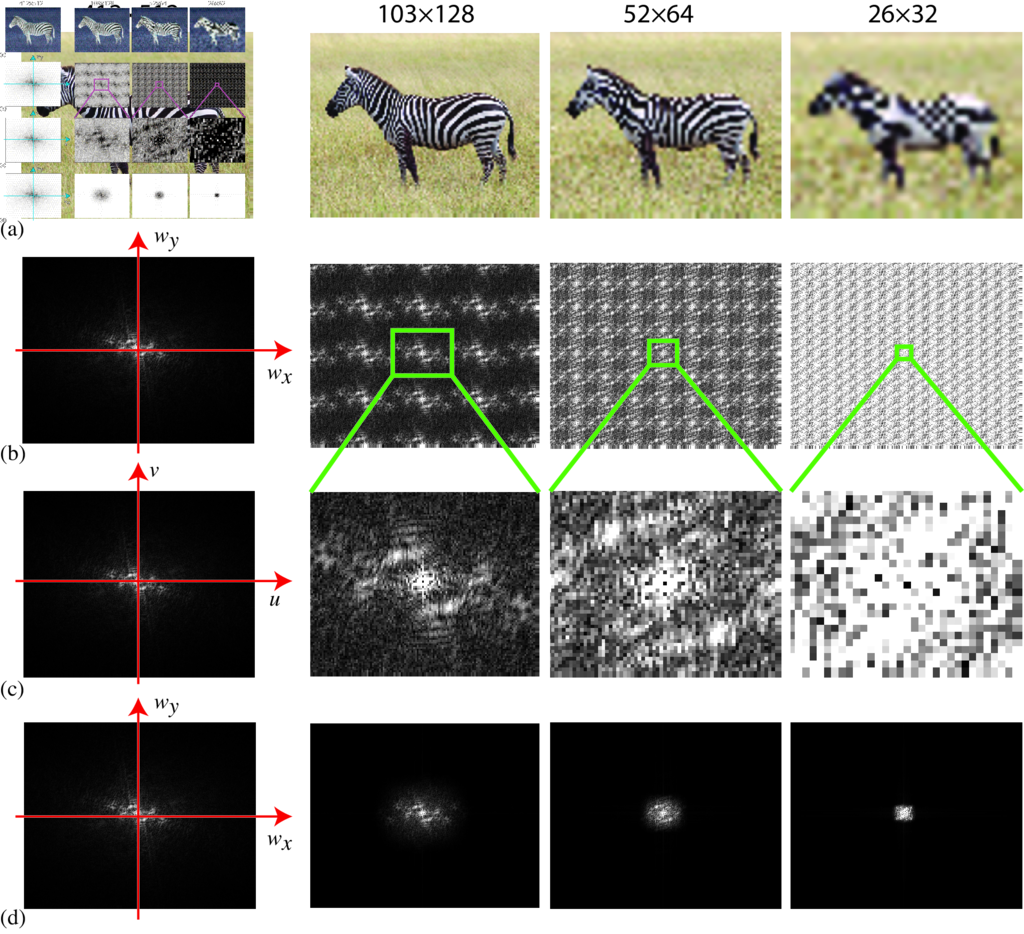
\includegraphics[width=1\linewidth]{figures/Image_processing_sampling/aliasing_ft_abc1.eps}
    \caption{Subsampling with aliasing. (a) The zebra sampled with aliasing starts looking like a cow. (b) Fourier transform of the continuous signal $\img(x,y)$ multiplied by delta trains: $\img_{\delta}(x,y)$. (c) Discrete Fourier transform of the corresponding sampled signals, $\img\left[n,m\right]$. (d) Fourier transform of the reconstructed signal with aliasing. (e) Sampled image after processing it with an anti-aliasing filter. (f) Discrete Fourier transform of the corresponding anti-aliased sampled images, $\img\left[n,m\right]$. Note that now the central part of the Fourier transform is not changing.
    }
    \label{fig:aliasingFTzebra}
\end{figure}


In order to reduce aliasing artifacts we need to filter the continuous signal with a low-pass filter in order to make it band-limited. Then we will be able to sample it avoiding high-spatial frequencies to interfere with the low-frequency content of the image. The anti-aliasing filter will not prevent the loss of information contained in the high spatial frequencies.  \Fig{\ref{fig:aliasingFTzebra2}}{a} shows the reconstructed images at different resolutions when an anti-aliasing filter is applied before sampling. Each resolution requires a different filter. The anti-aliasing filter can be a box filter like in \eqn{\ref{eq:boxfilterFT}} with the support equal to the green region in \fig{\ref{fig:aliasingFTzebra}}{b}.

\begin{figure}
    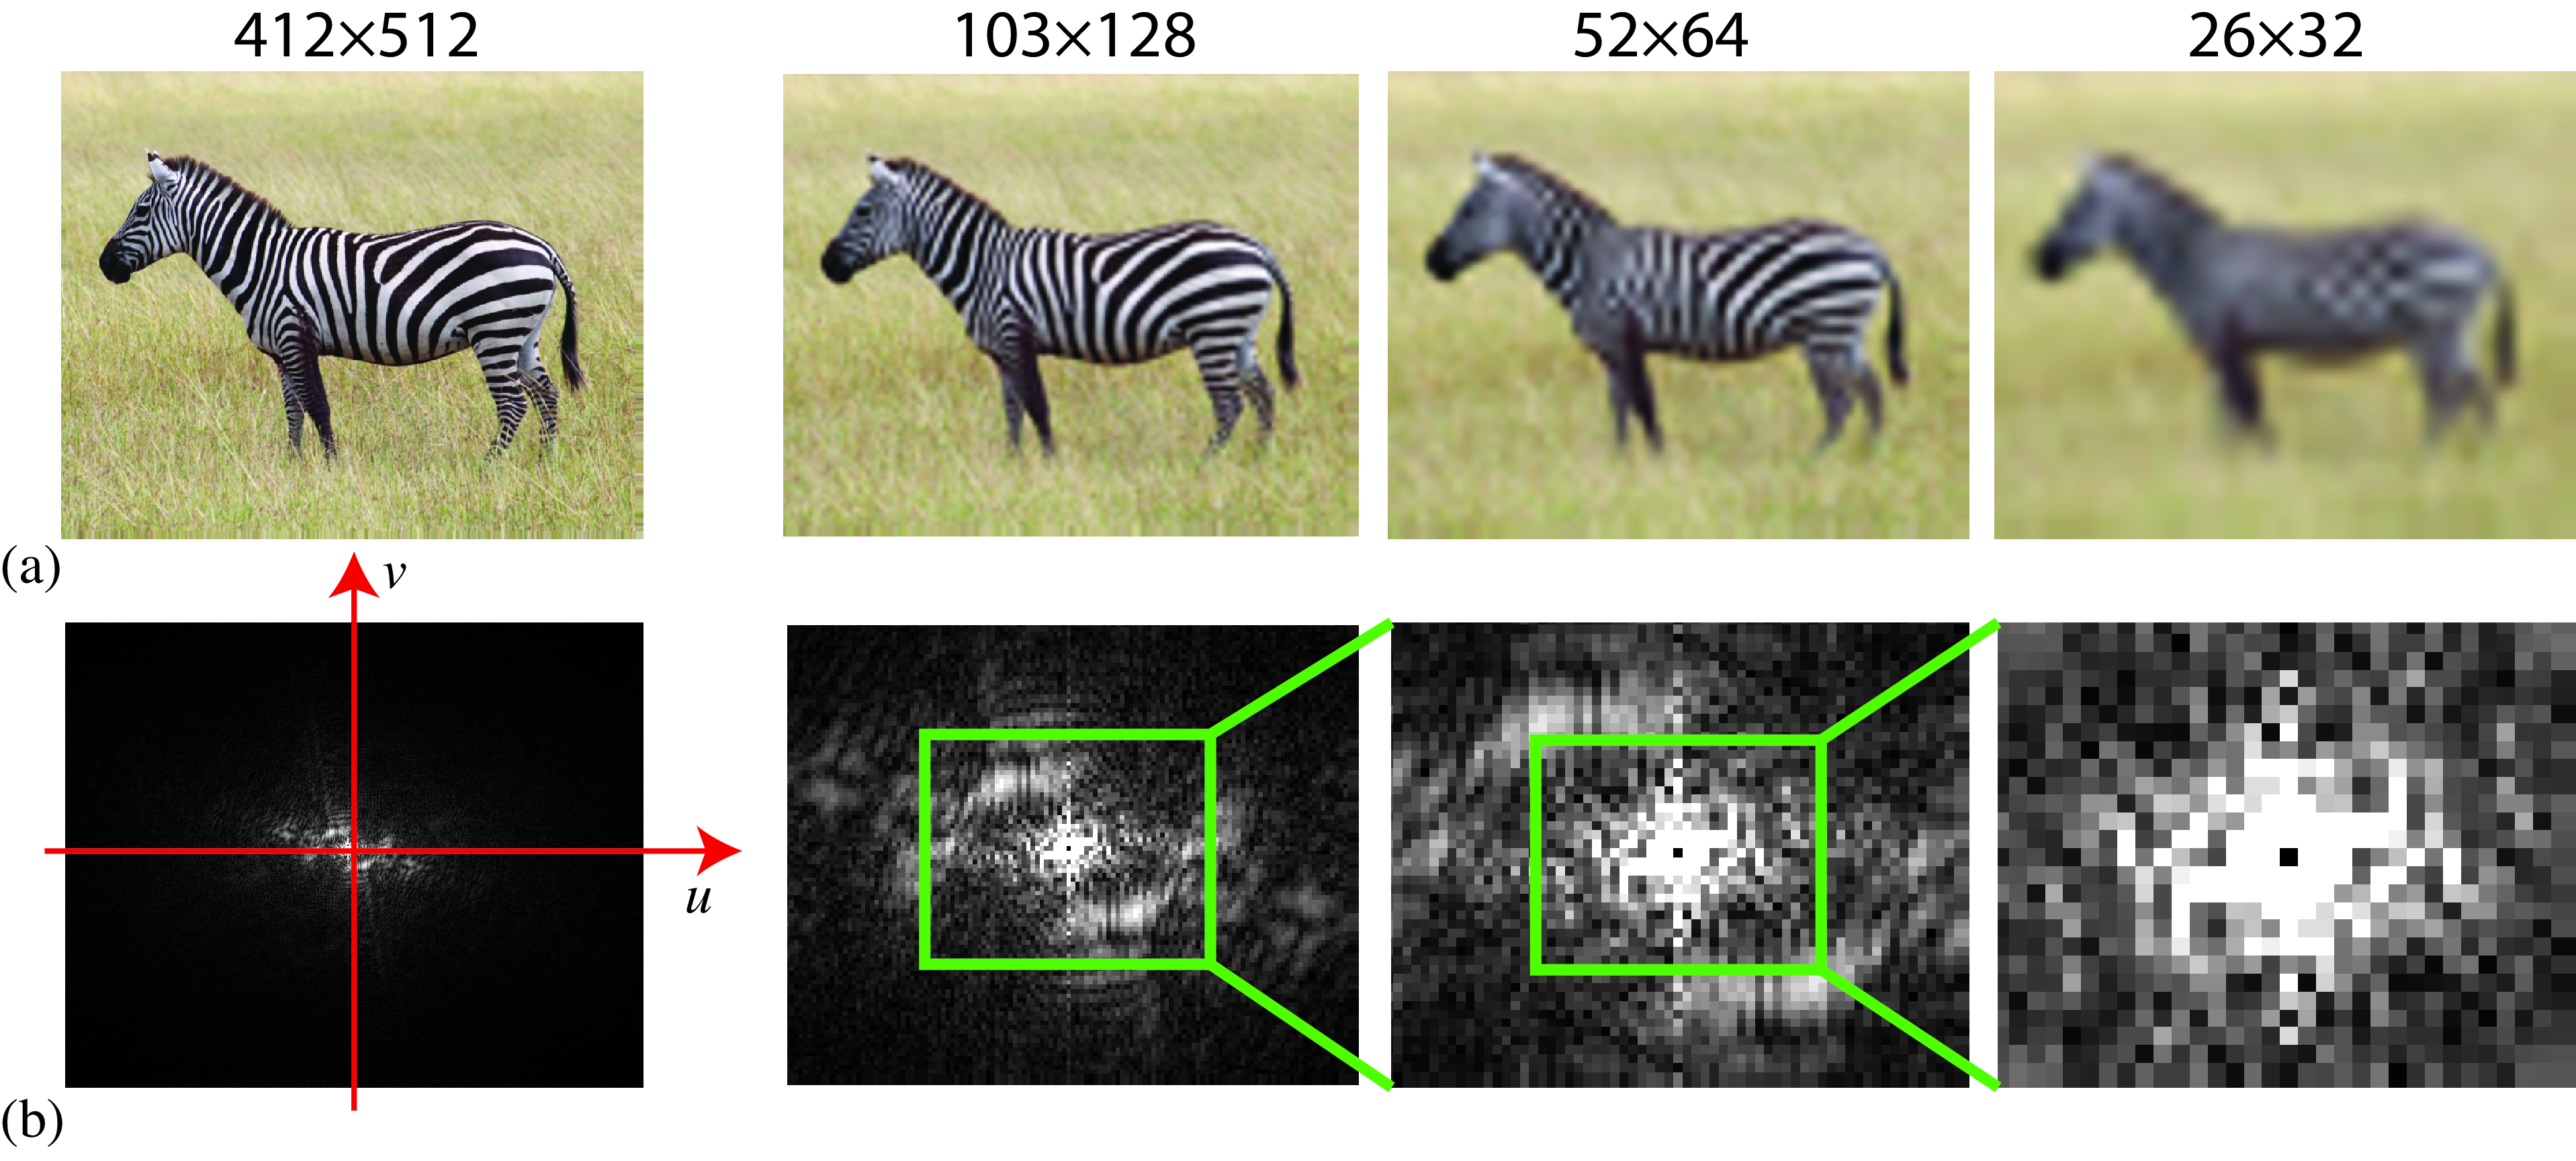
\includegraphics[width=1\linewidth]{figures/Image_processing_sampling/aliasing_ft_abc2.eps}
    \caption{Subsampling with anti-aliasing filter. (a) Sampled image after processing it with an anti-aliasing filter. (b) Discrete Fourier transform of the corresponding anti-aliased sampled images, $\img\left[n,m\right]$. Note that now the central part of the Fourier transform is almost not changing.
    }
    \label{fig:aliasingFTzebra2}
\end{figure}


%What are the sampling strategies used by biological systems. 
%
%
%Example in 2D:
%
%% https://pixabay.com/en/queen-cup-honeycomb-honey-bee-337695/
%
%Antialiasing filter
%
%
%FIGURE: show aliasing: a) show case of an image with an oriented wave and how aliasing makes the wave look as having a different frequency and orientation. b) show a 3D tilted wave and how near the horizon it creates a weird effect due to bad sampling.
%
%Types of 2D sampling: rectangular, hexagonal, random (There is a paper by Larry Maloney about this.). Aliasing patterns.
%
%2D antialiasing filter
%
%Sampling in biological systems.
%


\section{Spatiotemporal Sampling}

%\reviewcomment{References missing.}

Spatiotemporal sampling can be studied with the tools we have already seen. In particular, \eqn{\ref{eq:genericsampling}} can explain sampling in the $N$-dimensional case. Temporal aliasing is responsible of the typical illusion in which we see wheels or fans changing the sense of rotation in movies. To avoid those artifacts it is important to apply an anti-aliasing filter as before.

%There are many strategies commonly used to sample movies and each one has different advantages/disadvantages in terms of hardware implementation, efficiency, etc.

The most common type of spatiotemporal sampling is regular sampling: here, all the pixels are sampled in a regular spatial 2D grid and at regular time instants in which all the pixels are exposed simultaneously. This is also called global shutter mode.

In many cameras (DSLRs, mobile phones, etc.) the most commonly used sampling is the rolling shutter mode. Here, every row in the image is sampled simultaneously. But different rows are sampled at different instants. This sampling mode allows for a faster sampling rate with current hardware implementations but it can create spatial distortions in the image if the camera moves or when taking pictures of moving objects.

%- Examples of temporal aliasing
%
%Types of temporal sampling:
%
%- interlaced
%
%
%Global Shutter mode, every pixel is exposed simultaneously at the same instant in time
%Rolling shutter: The result is that each row in a frame will expose for the same amount of time but begin exposing at a different point in time, often produces undesirable skewing artifacts in recorded images, especially for photographs of moving objects




\section{Concluding Remarks}
%\reviewcomment{To be written.}

Aliasing is a common artifact that appears whenever an image is captured by sampling a continuous light field. As we will discuss in the next chapter, aliasing also affects images whenever there is upsampling or downsampling. Therefore, understanding how aliasing introduces artifacts and the best way to avoid it is an important skill.

However, aliasing is not always bad and it might be possible to use aliasing to recover high-frequency content that would be otherwise lost. Superresolution algorithms can learn to extract, from the aliasing pattern, fine image details.

Also, when an image is encoded by multiple channels, aliasing in one channel does not mean that the information is lost because multiple channels could contain complementary information that allows the recovery of high resolution details.

\marginnote{{\bf Moire patterns}, also related to aliasing, are interference patterns that appear when superposing semitransparent patterns on top of each other.
    \\[6pt]
    \centerline{
        \includegraphics[width=.4\linewidth]{figures/upsamplig_downsampling/moire.eps}
    }
}[-.5in]
\index{Moire pattern}